\chapter{Introduction}
\thispagestyle{empty}

On 5 July, 2022, in Helsinki, Finland, the International Mathematical Union announced the names of the four mathematicians who were to be awarded the Fields Medal, the most coveted prize in the world of mathematics: Hugo Duminil-Copin, June Huh, James Maynard and Maryna Viazovska. Duminil-Copin, Huh and Maynard received this most prestigious honour for making several outstanding contributions to their specific fields of expertise---respectively, statistical physics, geometric combinatorics, and analytic number theory. Viazovska, on the other hand, received the Fields Medal for more interdisciplinary achievements. Arguably the most remarkable of these was her solution to the sphere packing problem in dimension 8 \cite{Viazovska8}. It is difficult to place her solution in a specific mathematical field: what makes it so revolutionary is that it uses insights from Fourier analysis and the theory of modular forms to construct a special function---the Magic Function---that, in combination with a previous result by Cohn and Elkies \cite{CohnElkies}, proves that the $E_8$ lattice packing is the densest possible sphere packing in $\R^8$. Very shortly afterwards, Cohn, Kumar, Miller, Radchenko and Viazovska were able to use similar ideas to prove that the Leech lattice packing is the densest possible sphere packing in $\R^{24}$ \cite{Viazovska24}.

Before Viazovska's remarkable breakthrough, the optimal sphere packing density was only known in dimensions $1$, $2$ and $3$ \cite{CohnOnViazovska}. Furthermore, Thomas Hales' solution in dimension $3$ \cite{HalesKeplerInformal} was lengthy and involved extensive computer-assisted calculations; in contrast, Viazovska's proof in dimension $8$ is elegant and concise. 

% Say something here

\section{The Sphere Packing Problem}\label{Ch1:Sec:1_1_Sphere_Packing}

The Sphere Packing problem is a classical optimisation problem in mathematics. It goes as follows.

\begin{boxproblem}[The Sphere Packing Problem in Dimensinon $n$]\label{Ch1:Prob:SpherePacking_n}
    For some $n \in \N$, what is the densest non-overlapping arrangement of $n$-spheres of equal radius in $\R^n$?
\end{boxproblem}

Despite its straightforward formulation, \Cref{Ch1:Prob:SpherePacking_n} is notoriously difficult to solve. A key challenge in high dimensions is the fact that proceeding inductively is not always helpful: `stacking' the optimal $n$-dimensional sphere packing onto itself is not guaranteed to yield the optimal sphere packing in $n + 1$ dimensions~\cite{CohnOnViazovskaICM}. In fact, this appraoch is known to fail in dimensions as low as $10$~\cite{CohnOnViazovskaAMS}. This is not obvious, not least because the approach does, in fact, succeed in the visualisable dimensions of $1$, $2$ and $3$.

The $1$-dimensional case is uninteresting. Visually, one can easily see that the densest possible arrangement of disjoint intervals of the form $\parenth{-r, r}$ on the real line consists of intervals centred at all points $2rm$ for $m \in \Z$. Indeed, one can fix $r$ to be $\frac{1}{2}$ by rescaling the real line. The optimal packing therefore consists of open intervals of unit length centred at points on the lattice $\Z \subset \R$.

\begin{figure}[htb]
    \centering
    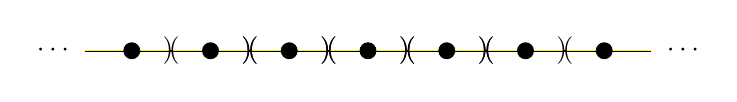
\begin{tikzpicture}
        \draw[step=1, black, thick] (-3.6, 0) -- (3.6, 0);
        \draw[yellow] (-3.6, 0) -- (-2.51, 0);
        \draw[yellow] (2.51, 0) -- (3.6, 0);
        \foreach \x in {-2, -1, 0, 1, 2} {
            \draw[yellow] (\x - 0.49, 0) -- (\x + 0.49, 0);
            \node at (\x - 0.5, 0) {$)\!($};
            \node at (\x + 0.5, 0) {$)\!($};
            \draw[fill=black] (\x, 0) circle (0.1);
        }
        \foreach \x in {-4, 4} {
            \node at (\x,0) {$\cdots$};
        }
        \draw[fill=black] (-3, 0) circle (0.1);
        \draw[fill=black] (3, 0) circle (0.1);
    \end{tikzpicture}
    \caption{The $\Z$ lattice packing in dimension $1$.}
    \label{Ch1:Fig:Z_Lattice_Packing_1D}
\end{figure}

In dimension $2$, \Cref{Ch1:Prob:SpherePacking_n}, also known as the circle packing problem, turns out to be more interesting. A reasonable strategy for finding the densest packing is to `stack' the $\Z$ lattice packing from dimension $1$ onto itself in some manner, turning these intervals into circles of the same radius. The question remains how to do this optimally.

One natural way of doing this is to stack the circles on top of themselves, turning $\Z$ into the lattice $\Z^2$, where circles are centred at points with integer coordinates: see \Cref{Ch1:Subfig:Z2_lattice_packing_2D}. Unfortunately, this packing turns out to be sub-optimal. A better candidate is the $A_2$ lattice packing: see \Cref{Ch1:Subfig:A2_lattice_packing_2D}. This packing is sometimes referred to as the \textit{honeycomb packing} due to the fact that every circle has six neighbours, whose centres form the vertices of a regular hexagon.

It is well-known that the honeycomb packing is optimal in $\R^2$. The original proof of this fact is attributed to Thue \cite{Thue}, but there are many proofs in the literature. One is outlined by Hales in \cite[p. 442]{CannonHoney}. An intuitive way of convincing oneself of Thue's theorem is that it is not possible for a circle in a given row to be in contact with more than $2$ circles in the rows above and below, meaning the $A_2$ packing cannot be improved. See \Cref{Ch1:Subfig:Kepler_Original_1}.

\begin{figure}[htb]
    \centering
    \begin{subfigure}{0.48\linewidth}
        \centering
        \begin{tikzpicture}[scale=1.25]
            \drawplane
            \foreach \x in {-2, -1, 0, 1, 2} {
                \foreach \y in {-2, -1, 0, 1, 2} {
                    \latticecircle{\x}{\y}
                }
            }
            \draw[->, color=brown, thick] (0,0) -- (1,0) node[anchor=north] {$\parenth{1, 0}$};
            \draw[->, color=brown, thick] (0,0) -- (0,1) node[anchor=east] {$\parenth{0, 1}$};
        \end{tikzpicture}
        \subcaption{The $\Z^2$ lattice packing.}
        \label{Ch1:Subfig:Z2_lattice_packing_2D}
    \end{subfigure}
    \begin{subfigure}{0.48\linewidth}
        \centering
        \begin{tikzpicture}[scale=1.25]
            \drawplane
            \clip (-2.5, -2.5) rectangle ++(5, 5);
            \foreach \x in {-4, -3, -2, -1, 0, 1, 2, 3, 4} {
                \foreach \y in {-3, -2, -1, 0, 1, 2, 3} {
                    \latticecircle{\x - \y * 0.5}{\y * 0.8660254038}
                }
            }
            \draw[->, color=brown, thick] (0,0) -- (1,0) node[anchor=north] {$\parenth{1, 0}$};
            \draw[->, color=brown, thick] (0,0) -- (-0.5,0.8660254038) node[anchor=south east] {$\parenth{-\frac{1}{2}, \frac{\sqrt{3}}{2}}$};
        \end{tikzpicture}
        \subcaption{The $A_2$ lattice packing.}
        \label{Ch1:Subfig:A2_lattice_packing_2D}
    \end{subfigure}
    \caption{Circle packings covering the square $\setst{\parenth{x, y} \subset \R^2}{-2.5 \leq x, y \leq 2.5}$.}
    \label{Ch1:Fig:Circle_Packings_2D}
\end{figure}

In dimension $3$, too, it is tempting to replicate this strategy: we can stack the $A_2$ packing on top of itself, in layers instead of rows, attempting to maximise the number of neighbours of a sphere. From trial and error, we see that a sphere cannot be in contact with more than three neighbours from the layer below. This suggests that the optimal sphere packing in dimension $3$ is given by stacking honeycomb arrangements on top of each other with spheres in each layer being nestled in the gaps between three spheres in the layer below.

\begin{wrapfigure}[28]{r}{0.27\linewidth}
    \centering
    \begin{subfigure}{\linewidth}
        \centering
        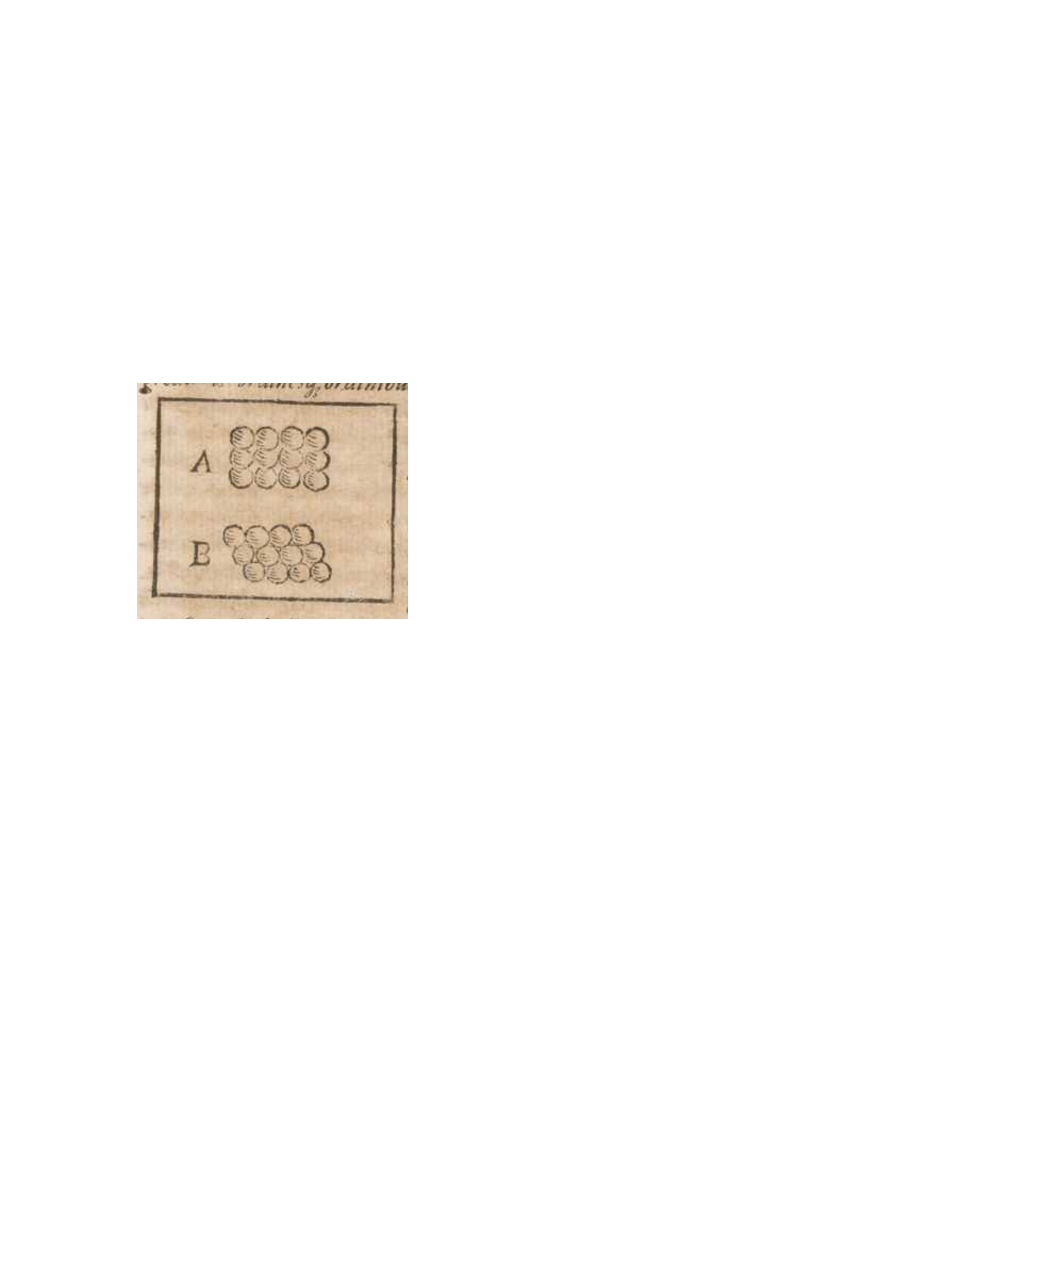
\includegraphics[width=\linewidth]{Chapters/1_Intro/Images/Kepler_1.pdf}
        \caption{}
        \label{Ch1:Subfig:Kepler_Original_1}
    \end{subfigure}
    \begin{subfigure}{\linewidth}
        \centering
        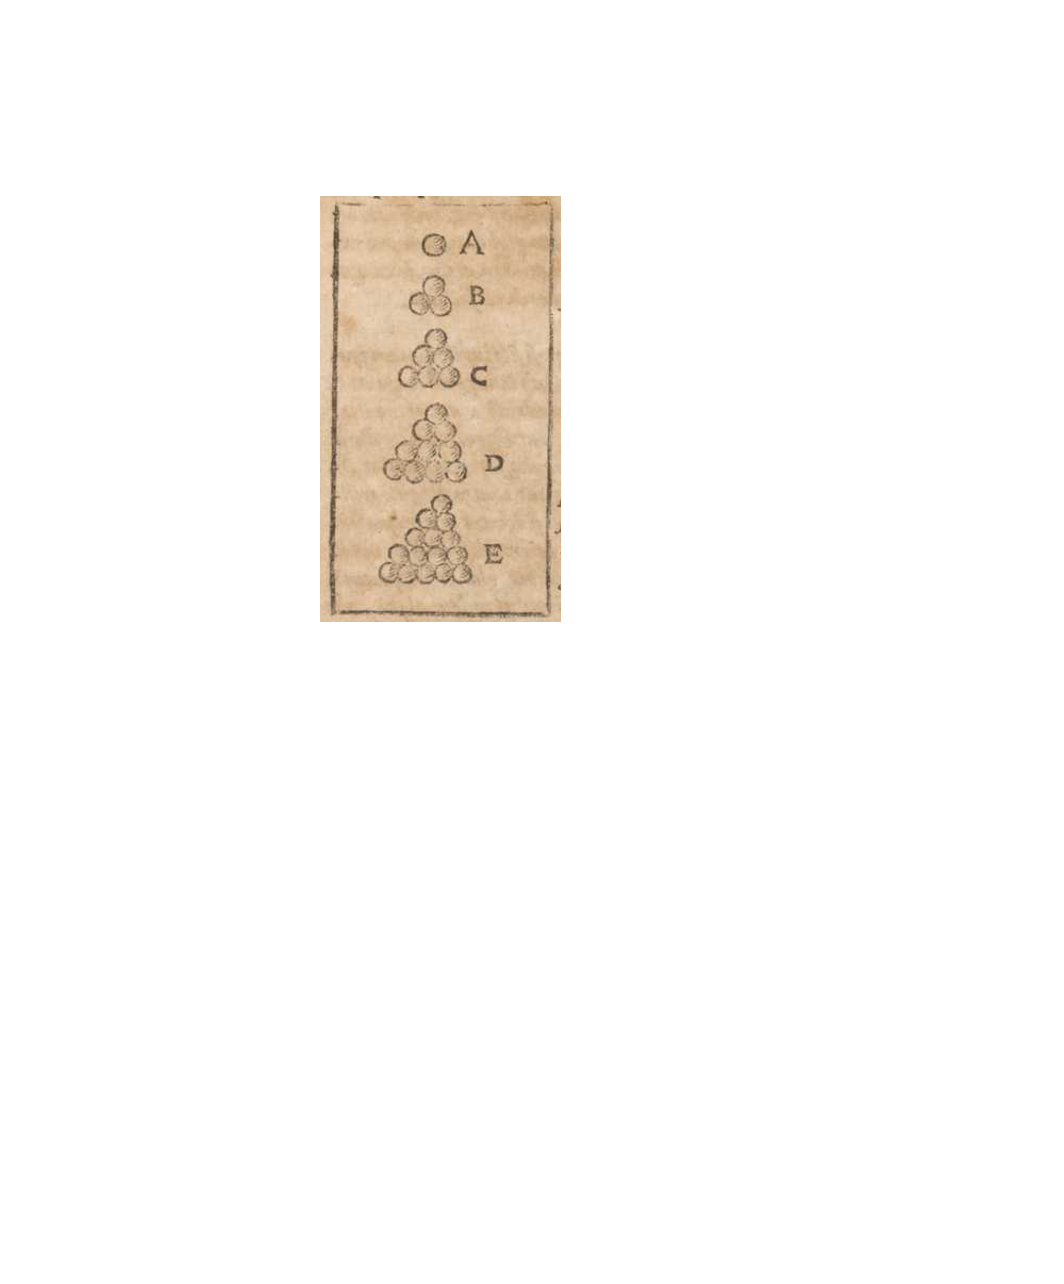
\includegraphics[width=\linewidth]{Chapters/1_Intro/Images/Kepler_2.pdf}
        \caption{}
        \label{Ch1:Subfig:Kepler_Original_2}
    \end{subfigure}
    \caption{Diagrams from an essay written by Johannes Kepler in Latin in 1611 \cite{KeplerSnowflake}.}
\end{wrapfigure}

As it turns out, unlike dimension $2$, this characterisation not describe a unique packing: spheres are simply too large! See \Cref{Ch1:Fig:2_Optimal_3D_Packings}. One can construct infinitely many locally similar, globally different sphere packings in $\R^3$, all of which are as dense as possible, by varying how successive layers are placed.

\begin{figure}[bt]
    \centering
    \begin{subfigure}{0.48\linewidth}
        \centering
        \begin{tikzpicture}[scale=1.25]
            \clip (-2.5, -2.5) rectangle ++(5, 5);
            \foreach \x in {-4, -3, -2, -1, 0, 1, 2, 3, 4} {
                \foreach \y in {-3, -2, -1, 0, 1, 2, 3} {
                    \latticecircle{\x - \y * 0.5}{\y * 0.8660254038}
                }
            }
            \foreach \x in {-3, -2, -1, 0, 1, 2} {
                \foreach \y in {-3, -2, -1, 0, 1, 2} {
                    \latticecirclegrey{\x - \y * 0.5}{\y * 0.8660254038 + 0.5773502692}
                }
            }
            \foreach \x in {-2, -1, 0, 1} {
                \foreach \y in {-2, -1, 0, 1} {
                    \latticecirclebrown{\x - \y * 0.5}{\y * 0.8660254038}
                }
            }
        \end{tikzpicture}
        \subcaption{}
        \label{Ch1:Subfig:3D_Triangular_Stacking}
    \end{subfigure}
    \begin{subfigure}{0.48\linewidth}
        \centering
        \begin{tikzpicture}[scale=1.25]
            \clip (-2.5, -2.5) rectangle ++(5, 5);
            \foreach \x in {-4, -3, -2, -1, 0, 1, 2, 3, 4} {
                \foreach \y in {-3, -2, -1, 0, 1, 2, 3} {
                    \latticecircle{\x - \y * 0.5}{\y * 0.8660254038}
                }
            }
            \foreach \x in {-2, -1, 0, 1, 2, 3} {
                \foreach \y in {-2, -1, 0, 1, 2, 3} {
                    \latticecirclegrey{\x - \y * 0.5}{\y * 0.8660254038 - 0.5773502692}
                }
            }
            \foreach \x in {-2, -1, 0, 1} {
                \foreach \y in {-2, -1, 0, 1} {
                    \latticecirclebrown{\x - \y * 0.5}{\y * 0.8660254038 + 0.5773502692}
                }
            }
        \end{tikzpicture}
        \subcaption{}
        \label{Ch1:Subfig:3D_Hexagonal_Stacking}
    \end{subfigure}
    \caption{Two different ways of stacking the honeycomb packing on itself.}
    \label{Ch1:Fig:2_Optimal_3D_Packings}
\end{figure}

This observation is not novel. In a 1611 essay whose title has been translated from Latin as \textit{The Six-Cornered Snowflake} \cite{KeplerSnowflake}, Johannes Kepler asserted that spheres cannot be more tightly packed together than they are in a tetrahedral arrangement: see \Cref{Ch1:Subfig:Kepler_Original_2}. This result became known as the Kepler Conjecture, and it went unproven for over three centuries, until 2005 that a paper proving it, written by Thomas Hales, was published \cite{HalesKeplerInformal}.

The complexity of the sphere packing problem in dimension $3$ is illustrated not only by the time elapsed between Kepler's original assertion and a proof being published but also by the length of Hales's paper. Indeed, in an expository account of his proof published in 2000, five years before the publication of the full paper in the Annals, Hales recounted how a jury of twelve referees, despite having been in deliberation for over a year, had yet to make a ``thorough, independent check of the computer code'' he had written to perform the elaborate calculations on which ``every aspect of [his proof] is based'' \cite{CannonHoney}. In January 2003, at the Joint Math Meetings in Baltimore, USA, Hales announced that he intended to formally verify his proof \cite{HalesKeplerFormal}, in what he termed the Flyspeck project. The paper authored by Hales and his collaborators on their successful formalisation of his argument was only published in 2017. Therefore, not only did the Kepler Conjecture take close to 400 years to solve, but it took nearly two decades to eliminate any doubt as to the correctness of the solution. This project aims to formalise a result of a similar flavour in a significantly shorter timeframe.
\section{The Work of Maryna Viazovska}
\section{The Formalisation Movement}
\section{Progress in Formalising Viazovska's Solution in Dimension $8$}

% Do I want to turn this into a separate chapter and toss in section 1.5?
\section{The Scope of this Project}